\documentclass[tikz,border=2mm]{standalone}
\usetikzlibrary{arrows.meta}
\usepackage{amsmath}

\begin{document}
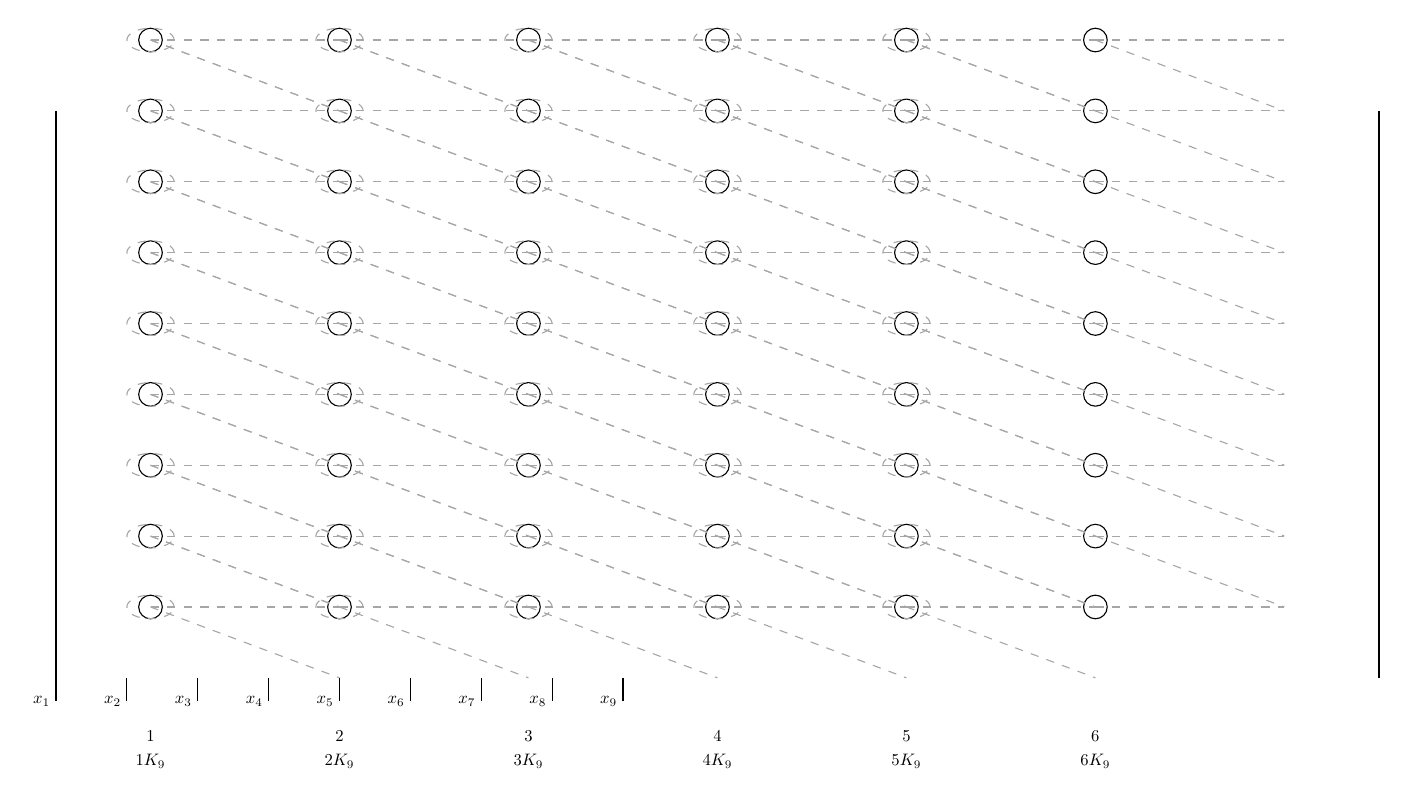
\begin{tikzpicture}[scale=0.6, transform shape]

% Draw horizontal lines
\foreach \i in {1,...,9}
{
  \pgfmathsetmacro{\ypos}{(\i-1)*1.5}
  \draw (\ypos, 0) -- ++(0,-0.5) node[left]{$x_{\i}$};
}

% Draw vertical lines
\draw[thick] (0, 12) -- (0, 0);
\draw[thick] (28, 12) -- (28, 0);

% Draw nodes and ellipses
\def\n{9} % Number of nodes per row
\def\m{6} % Number of columns
\foreach \j in {1,...,\m}
{
  \foreach \i in {1,...,\n}
  {
    \pgfmathsetmacro{\xpos}{(\j-1)*4 + 2}
    \pgfmathsetmacro{\ypos}{(\n-\i+1)*1.5}
    \pgfmathsetmacro{\label}{\j*\n-\i+1}
    \filldraw[circle, fill=white, draw=black, thin] (\xpos, \ypos) circle (0.25);
    \ifnum\j<\m
      \draw[dashed, gray!70] (\xpos, \ypos) ellipse (0.5 and 0.25);
    \fi
  }
}

% Label rows
\foreach \k in {1,...,\n}
{
  \pgfmathsetmacro{\ypos}{(\n-\k+1)*1.5}
  \draw (\ypos, -1) node[below]{};
}

% Label columns
\foreach \l in {1,...,\m}
{
  \pgfmathsetmacro{\xpos}{(\l-1)*4 + 2}
  \node[below] at (\xpos, -1) {\l};
}

% Draw arcs
\foreach \j in {1,...,\m}
{
  \foreach \i in {1,...,\n}
  {
    \pgfmathtruncatemacro{\nextcol}{\j+1}
    \pgfmathtruncatemacro{\nextrow}{\i+1}
    \pgfmathsetmacro{\xstart}{(\j-1)*4 + 2}
    \pgfmathsetmacro{\ystart}{(\n-\i+1)*1.5}
    \pgfmathsetmacro{\xend}{\j*4 + 2}
    \pgfmathsetmacro{\yend}{(\n-\i+1)*1.5}
    
    % Horizontal dashed line between same row
    \draw[dashed, gray!70] (\xstart, \ystart) -- (\xend, \yend);
    
    % Diagonal dashed lines between adjacent rows
    \ifnum\i<\n
      \pgfmathsetmacro{\ynext}{(\n-\nextrow+1)*1.5}
      \draw[dashed, gray!70] (\xstart, \ystart) -- (\xend, \ynext);
    \fi
    
    % Vertical dashed lines within same column
    \ifnum\j<\m
      \pgfmathsetmacro{\xnext}{\j*4 + 2}
      \pgfmathsetmacro{\yend}{(\n-\i+1)*1.5}
      \pgfmathsetmacro{\ynext}{(\n-\nextrow+1)*1.5}
      \draw[dashed, gray!70] (\xstart, \ystart) -- (\xnext, \ynext);
    \fi
  }
}

% Label column titles
\foreach \k in {1,...,\m}
{
  \pgfmathsetmacro{\xpos}{(\k-1)*4 + 2}
  \node[below=1.5cm] at (\xpos, 0) {$\k K_9$};
}

\end{tikzpicture}
\end{document}